% -*- mode: LaTex; outline-regexp: "\\\\section\\|\\\\subsection";fill-column: 90; -*-
\documentclass{gSCS2e}   
% \documentclass[12pt]{article}\usepackage[longnamesfirst]{natbib}
\usepackage[usenames]{color}
\usepackage{graphicx}    % Macintosh pdf files for figures
\usepackage{bbm}            % one symbol
\usepackage{amssymb}   % Real number symbol {\Bbb R}
\input{../../standard}
  
% --- margins
% \usepackage{../../sty/simplemargins}
% \setleftmargin{1in}   % 1 inch is NSF legal minimum
% \setrightmargin{1in}  % 1 inch is NSF legal minimum
% \settopmargin{1in}    % 1 inch is NSF legal minimum
% \setbottommargin{1in} % 1 inch is NSF legal minimum

% --- Paragraph split, indents
% \setlength{\parskip}{0.00in}
% \setlength{\parindent}{0in}

% --- Line spacing
\renewcommand{\baselinestretch}{1.8}

% --- Margins
% \setlength{\topmargin}{-0.5in}
% \setlength{\oddsidemargin}{-0.1in}
% \setlength{\textheight}{9.0in}
% \setlength{\textwidth}{6.5in}

% --- page numbers
% \pagestyle{empty}  % so no page numbers

% --- Hypthenation
\sloppy  % fewer hyphenated
\hyphenation{stan-dard}
\hyphenation{among}

% --- Customized commands, abbreviations
\newcommand{\TIT}{{\it  {\tiny Risk of sequential tests (\today)}}}

\newcommand{\test}{\mbox{$\hat\mu(\al(\cdot),W_0,\omega)$}}
\newcommand{\uTest}{\mbox{$\hat\mu(\al_u(\cdot),W_0,\omega)$}}
\newcommand{\gTest}[1]{\mbox{$\hat\mu(\al_g(\cdot,{#1}),W_0,\omega)$}}

% --- Header
% \pagestyle{myheadings}
% \markright{\TIT}

% --- Title

\title{ Risk Inflation of Sequential Tests \\ Controlled by Alpha Investing }
\author{
        Dean P. Foster and Robert A. Stine
        \thanks{Research supported by NSF grant DMS-1106743 }  \\
        Department of Statistics            \\
        The Wharton School of the University of Pennsylvania \\
        Philadelphia, PA 19104-6340           
}

\date{\today}


%%%%%%%%%%%%%%%%%%%%%%%%%%%%%%%%%%%%
% something about submission problem
% \pdfminorversion=4 


\begin{document}
\maketitle 
%------------------------------------------------------------------------
\vspace{-0.2in}
\abstract{ 

 Streaming feature selection is a  greedy approach to variable selection that evaluates
 potential explanatory variables sequentially.  It selects significant features as soon as
 they are discovered rather than testing them all and picking the best one.  Because it is
 so greedy, streaming selection can rapidly explore large collections of features.  If
 significance is defined by an alpha investing protocol, then the rate of false
 discoveries will be controlled.  The focus of attention in variable selection, however,
 should be on fit rather than hypothesis testing.  Little is known, however, about
 the risk of estimators produced by streaming selection and how the configuration of these
 estimators influences the risk.  To meet these needs, we provide a computational
 framework based on stochastic dynamic programming that allows fast calculation of
 the minimax risk of a sequential estimator relative to an alternative.  The alternative
 can be data-driven or derived from an oracle.  This framework allows us to compute and
 contrast the risk inflation of sequential estimators derived from various alpha investing
 rules.  We find that a universal investing rule performs well over a variety of models
 and that estimators allowed to have larger than conventional rates of false discoveries
 produce generally smaller risk.

}

%------------------------------------------------------------------------
\vspace{0.05in}

\noindent
{\it Key Phrases: stochastic dynamic programming, testimator, variable selection}

\clearpage


% ----------------------------------------------------------------------
\section{ Introduction }
% ----------------------------------------------------------------------

 Our analysis concerns the risk of sequential estimators in which characteristics of later
 estimators depend on earlier estimates.  Our interest in the risk of such estimators
 arises from their use in streaming feature selection.  Streaming feature selection
 constructs a predictive model by greedily choosing explanatory variables from a sequence
 offered by an exogenous source.  Think of forward stepwise regression, but without
 knowledge of the complete domain of explanatory variables.  Rather than evaluate the
 collection of possible explanatory variables together, streaming selection evaluates them
 one-at-a-time.  Searches like stepwise regression consider the full batch of, say, $p$
 potential explanatory variables together, choosing at the first step the predictor
 $X_{(1)}$ that obtains the best fitting model.  In contrast, streaming selection is even
 more greedy and evaluates features sequentially as $X_1, \, X_2, \ldots$, judging $X_j$
 having observed $X_1, \ldots, X_{j-1}$.  Hence, streaming selection does not wait to
 examine every explanatory variable before making a selection.  It is also free to use the
 results of evaluating initial variables to guide the search for those to consider
 subsequently.  For example, a streaming search might test the interaction $X_j \, X_k$
 after finding significant effects for $X_j$ and $X_k$.  Streaming selection can thus
 adaptively explore collections of explanatory variables that are larger than typically
 considered with conventional methods. \citet{wu13} provide several examples, including
 image processing, in which streaming selection is valuable.  For large samples, the
 slowest step in forward stepwise regression is the calculation of the $X'X$ matrix.
  \citet{fosterlin11} demonstrate the speed attained by sequential selection when picking
 a regression from up to 100,000 explanatory variables.


 Streaming selection poses a challenge, however, for variable selection.  Although one
 gains advantages by avoiding simultaneously evaluating every predictor, the absence of a
 fixed set of features in streaming selection requires a different type of selection
 criterion from those commonly used.  For example, suppose the search begins with a list
 of $p$ potential features $X_1, X_2, \ldots, X_p$.  As mentioned, the search could expand
 to include interactions in $X_j$ once $X_j$ joins the model.  If the search were limited
 to second-order interactions, then the number of possible explanatory variables would
 become $m = p(p+1)/2$ variables.  One could go further and allow the sequential search to
 construct and test third and fourth-order interactions derived by interacting previously
 selected features and pairwise interactions. The resulting search would examine only
 those higher-order interactions that generate nontrivial lower-order
 interactions. Because higher-order interactions with non-zero effects typically have
 nontrivial lower-order projections \citep{kalai09}, this ``bottom-up'' search is likely
 to detect these interactions.  Even so, fourth-order interactions are likely to be very
 sparse, and the streaming search would likely examine only a few of these.  It would thus
 be conservative to combine this search with a criterion such as AIC or BIC that adds a
 penalty proportional to the size of the search space that would grow to $m = O(p^4)$.
  The penalties used in these criteria presume one examines all $m$ features rather than a
 dynamically chosen subset.  Similarly, selection using FDR requires the complete set of
 $m$ possible p-values at the start of the search.


 Alpha investing \citep{fosterstine08} is a sequential testing procedure
 that is well-suited to streaming feature selection.  Because alpha investing can
 test an infinite sequence of hypotheses, it is well-matched to a search of a
 possibly unbounded collection of features.  Rather than test multiple
 hypotheses at once, alpha investing tests hypotheses one-at-a-time in a
 specified order.  Alpha investing begins with an initial allowance for Type I
 error that is called its alpha wealth.  Each test consumes some of the
 available alpha wealth, as in alpha spending rules used in clinical trials.
  Alpha investing overcomes the conservatism of alpha spending rules, which
 include the Bonferroni method, by earning a contribution to the alpha wealth
 for each rejected null hypothesis.  Thus rejections beget more rejections.
  Alpha investing further allows one to test an infinite stream of hypotheses,
 accommodate dependent tests, and incorporate domain knowledge.
 

 Like other procedures for multiple testing, alpha investing controls the expected number
 of false rejections.  Controlling the false discovery rate protects against overfitting
 in variable selection.  One can guarantee that on average not more than, say, 5\% of the
 rejected hypotheses spuriously add a predictor to the model.  When building a predictive
 model, however, we find that controlling the false discovery rate is secondary to
 obtaining a more predictive model.  Control of the false discovery rate does not imply
 that one finds the most predictive model.  It only guarantees that a high percentage of
 chosen features are in fact useful.  The quadratic risk of the implied estimator is more
 relevant.  Furthermore, alpha investing is not one method, but rather a general approach
 to testing a sequence of hypotheses.  It offers a modeler a variety of choices that control
 how the procedure sets the level for the next test. The impact of these choices on the
 risk of the resulting model is by-and-large unknown.


 To study the risk of alpha investing estimators and the effects its tuning parameters, we
 convert the choice of features in regression into the classical normal means problem.
  Consider fitting the regression of $Y$, a vector of $n$ observations, on the linearly
 independent columns $X_1,\ldots,X_p$ that make up the $n\times p$ matrix $X$.  The
 Gram-Schmidt algorithm sequentially converts these explanatory variables into orthonormal
 variables $\tilde{X}_1,\ldots,\,\tilde{X}_p$.  In matrix form, the regression $Y = X
 \beta + \epsilon$ with $\ep_i \sim N(0,\sigma^2)$ becomes $Y = (X T)( T^{-1}\beta) +
 \epsilon = \tilde{X} \mu + \epsilon$, where $T$ is the upper triangular matrix defined by
 the Gram-Schmidt algorithm.  Multiplying both sides of this equation on the left by
 $\tilde{X}'$ produces
\begin{equation*}
   \tilde{X}'Y =  \tilde{Y}  = \mu + \tilde \epsilon \;,
\end{equation*}
 where $\tilde\epsilon = X'\epsilon \sim N(0,\sigma^2)$.  Evaluating which of
 $X_1,\ldots,X_p$ to add to the regression thus becomes a test of which of the first $p$
 elements of $\mu$ differ from zero.  \citet{lehmann05} (Chapter 7) describes this
 conversion in more detail. In practical implementations of sequential variable selection
 (such as \cite{fosterlin11}), one only sweeps selected features from those that remain,
 allowing $p > n$.
 
 
 The methods developed here find the cumulative risk of a sequence of testimators in the
 context of testing a sequence of means.  Rather than observe a sequence of slope
 estimates, we assume that the observed statistics are a sequence of $p$ random variables
 $Y_j \sim N(\mu_j,1)$.  A testimator is also known as a keep-or-kill estimator or a hard
 thresholding estimator.  The estimator of the parameter $\mu$ is zero unless $H_0: \,\mu
 = 0$ is rejected.  Within this context, our algorithm reveals the attainable risks of a
 testimator for {\em any} choice of parameters.  We accomplish this task by adopting the
 perspective of risk inflation and comparing the competitive performance of two sequential
 estimators.  For any pair, we find the set of attainable risks.  Given the sequential
 nature of the problem, it should not be surprising that we rely on stochastic dynamic
 programming.  The risks so obtained are exact (up to computational accuracy) rather than
 asymptotic.  We further show a probabilistic model for the underlying parameters that
 approximates those risks.  Although we consider sequential estimators, we find that
 bounds for the risk inflation of conventional testimators also characterize the risk of
 sequential testimators.


 The following section provides further introduction to alpha investing.  We
 derive two alpha investing strategies from continuous probability
 distributions.  Our construction of these strategies in Section 2 is novel and
 allows us to minimize the state space required in the dynamic program.  Section
 3 describes the risk of a sequence of testimators.  Section 4 defines the
 feasible set of possible risks and uses these to compare
 testimators to an oracle and to each other.  Section 5 describes the
 computations in more detail.  We conclude in Section 6 with a brief discussion
 of the results and pose conjectures motivated by our computations.



% ---------------------------------------------------------------------------
\section{ Alpha-investing }
% ---------------------------------------------------------------------------

 An alpha-investing rule \citep{fosterstine08} determines the levels for testing
 a sequence of hypotheses $H_1, \,H_2, \dots,$.  The procedure is most easily described
 by showing a few steps.  The process begins with an initial allocation $W_0 >
 0$ of alpha wealth.    An alpha-investing rule can test $H_1$ at
 any level $\al_1$ up to the initial alpha wealth, $0 \le \alpha_1 \le W_0$.
  The level $\al_1$ is `invested' and cannot be used for subsequent tests.  We
 say that $\al_1$ is invested rather than spent because rejecting $H_1$ produces an 
 increment in the alpha wealth, a return on the investment.  Let $p_1$ denote
 the p-value of the test of $H_1$.  If $p_1 \le \alpha_1$, the test rejects
 $H_1$, and the alpha investing rule earns a contribution $\omega \ge
 0$ to its alpha wealth.  Otherwise, the alpha wealth available to test $H_2$
 falls to $W_1 = W_0 - \alpha_1$.  In general, the alpha wealth available for
 testing $H_{j+1}$ is given by the stochastic process
 \begin{equation}
    W_j = W_{j-1} - \alpha_j + \omega \, I_{\{p_j \le \al_j\}}, 
       \quad j = 1,\,2,\ldots,
 \label{eq:Wj}
 \end{equation}
 with the initial condition that specifies the initial wealth $W_0$.  Alpha
 spending rules are alpha investing rules that constrain $\omega = 0$.


 Because rejecting a null hypothesis makes it easier to reject other null
 hypotheses, it is essential for alpha investing to control the rate of false
 rejections.  To this end, \citet{fosterstine08} show that alpha investing
 controls a sequential version of the expected false discovery rate, mFDR.  Let
 $T(j)$ count the number of hypothesis rejected among the first $j$ tests, and let
 $V(j) \le T(j)$ denote the total number of {\em false} rejections among the
 first $j$ tests.  The sequential mFDR is
 \begin{equation}
    \mbox{mFDR}_\eta(j) = \frac{\ev V(j)}{\eta + \ev T(j)} \;, \quad \eta > 0.
 \label{eq:mFDR}
 \end{equation}
 In contrast, FDR is the expected value of the ratio $V(j)/T(j)$ conditional on
 $T(j)>0$ rather than the ratio of expected values.  The constant $\eta$ in the
 denominator of mFDR avoids dividing by zero under the complete null
 hypothesis in which all $\mu_j = 0$.  If $W_0 \le \eta\,\omega$, then
 alpha-investing rules control $\mbox{mFDR}_\eta(p) \le \omega$, and this result
 implies weak control of the family wide error rate.  Because these properties
 of alpha investing originate in a martingale, the index $j$ in \eqn{mFDR} is
 allowed to be an arbitrary stopping time, such as the occurrence of the $k$th
 rejection.

 
 Alpha-investing rules are quite general.  The underlying theory requires only that the
 level of the test of $H_j$ is bounded by the available wealth $W_{j-1}$ and that the test
 indeed have level $\al_j$, conditional on the outcomes of prior tests.  Otherwise, an
 alpha investing rule can use the pattern of prior rejections.  We represent this
 dependence by writing an alpha investing rule ${\cal A}$ as a function of the sequence of
 prior wealths $W_{0:j-1} = \{W_0, W_1, \ldots, W_{j-1}\}$.  The rule $\cal A$ maps this
 history to the interval from zero to the current wealth:
 \begin{equation}
    {\cal A}: W_{0:j-1} \mapsto [0, \min(W_{j-1},1)]    
 \label{eq:A}
 \end{equation}
 For example, $\cal A$ can set the level of the next test higher or lower depending upon
 the number of tests since the last rejection or the accumulated number of rejections.
  Although alpha investing allows this generality, we focus on a simpler class of
 investing rules that have a path independent, Markovian structure.  The amount invested
 by these rules depends only on the current wealth rather than the full path, $\alpha_j =
 {\cal A}(W_{0:j-1}) = \al(W_{j-1})$.  The only requirement is that $0 \le \al(w) \le w$;
 a rule cannot invest more wealth than the amount possessed.  It does seem natural,
 however, for $\al(w)$ to be monotone increasing in $w$.


 \remark{ To avoid adding notation, we overload the symbol $\al$.  Throughout
 these uses, the symbol $\alpha$ consistently gives the level of a test; only
 the context of the test changes.  By itself, $\al$ represents the
 generic level of a test.  When given an integer subscript, $\al_j$ is the level
 of the $j$th test in sequence of tests, as in \eqn{Wj}.  Finally, denoting a
 function, $\al(w)$ is the level invested in a test by an alpha investing rule
 that has available wealth $w$, as in \eqn{Ageo} that follows.  }


 The simplest representatives of this class of alpha investing rules are
 geometric rules.  These invest a fixed percentage of the available wealth on
 each test:
 \begin{equation}
    \al_g(w, \psi) = \psi \, w, \quad  0 < \psi < 1.
 \label{eq:Ageo}
 \end{equation}
 Since the alpha wealth increases after a rejection (provided $\al_j < \omega$), a
 geometric rule $\al_g$ invests more following a rejection and then gradually -- at the
 rate determined by $\psi$ -- reduces the level of subsequent tests.


 Alternatively an alpha investing rule can vary the share of the current wealth
 to invest in the next test.  Rather than invest a fixed share of the available
 wealth, the following rule invests progressively less  as its wealth
 drops.  The rule is defined by
 \begin{equation}
   \al_u(w) = w - \frac{\log 2}{\log(1+2^{1/w})} \;.
 \label{eq:Auniv}
 \end{equation}
 Using the procedure described in the appendix, we derived $\alpha_u$ from the density function
  \begin{equation}
    A_u(x) = \frac{\log 2}{x (\log x)^2} \;, \quad 2 \le x \;.
    \label{eq:Au}
 \end{equation}
  $A_u$ is motivated by the penultimate binary code for representing positive integers defined by  
  \citet{elias75}.  This code is universal in the sense of producing compact representations for 
  data sampled from a variety of probability distributions, 
   and so we refer to $\al_u$ as a universal investing rule.
   
 \remark{ The structure of the penultimate code and its relationship to $A_u$ may be of
 independent interest.  Suppose that the random variable $X$ has a discrete distribution
 on the positive integers with $\pr(X = j) = p_j$ for $j = 1,\,2,\, \ldots$.  A code that
 represents $X$ using $-\log_2 p_{X}$ bits has the minimal expected length, which is given
 by the entropy of the distribution, $-\sum_{j=1}^n (\log_2 p_j) p_j = H_X$.  Hence, the
 shortest binary prefix code for an {\it iid} sequence $\{X_1,\ldots,X_n\}$ from this
 distribution has expected length $n\;H_X$.  Within this context, the penultimate code of
 Elias is asymptotically optimal and universal in the following sense.  Let $L(j)$ denote
 the length of the penultimate code for the integer $j$. So long as the probabilities
 $p_j$ are monotone decreasing, $p_j \ge p_k$ if $j \le k$, then $\lim_n \sum_{j=1}^n
 E\,L(X_j)/(n H_X) = 1$. That is, regardless of the choice of monotone probabilities, the
 expected length of the penultimate code lies within a constant factor of the length of
 the best possible code. The structure of the penultimate code is quite simple and leads
 to the expression \eqn{Au} for $A_u$.  The penultimate code for an integer $x$ contains
 the binary representation of $x$ which requires $b(x) \approx \log_2 x$ bits. To form a
 prefix code, this code includes a binary representation of $b(x)$ that requires about $2
 \log_2 b(x)$ additional bits.  Combining these, $L(x) \approx \log_2 x + 2 \log_2 \log_2
 x$.  This length suggests a probability distribution of the form $q(x) = c_q 2^{-L(x)} =
 c_q/(x \; \log(x)^2)$ with $c_q$ chosen so that $\sum_x q(x) = 1$. $A_u(x)$ is a
 continuous version of $q(x)$.  \citet{rissanen83} refined the penultimate code by
 incorporating a more efficient representation for $b(x)$ and labeled the result the
 universal code for integers.  For an extensive introduction to coding and its connections
 to statistics, see \citet{coverthomas06}.  }

  
  
 Figure \ref{fig:rules} contrasts the investments of the universal and several geometric
 alpha investing rules.  The figure conveys the sense in which $\al_u$ is universal in the
 way that it mimics a collection of geometric rules.  For convenience, the initial wealth
 for all rules shown in Figure \ref{fig:rules} is $W_0 = 1$.  On a log-log scale, the
 amounts invested by the universal rule fall off approximately linearly.  These amounts
 are initially larger than those of any of the geometric rules.  Starting from $W_0=1$,
 the universal rule invests about $0.369$, $0.131$, $0.0693$, $0.0438$, and $0.0306$ in
 the first five tests before its spending gradually slows.  After this initial period,
 there is a range of tests over which each geometric rule invests the largest alpha level.
  For tests in this range, that rule is the most able to find signal. The universal rule
 invests almost as much as each geometric rule when that rule invests the most, and
 ultimately, the universal rule invests more.  For example, the geometric rule that
 invests 1\% of its wealth at each test ($\psi=0.01$) invests more than the universal rule
 when testing $H_{11}$ through $H_{581}$; otherwise it invests less.  The graph shows that
 the universal rule saves enough so that it can spend close to the rate of the maximal
 geometric.

 % Too bad we don't have that 'habitation' idea worked out where the universal
 % finds a steady rate appropriate for the rate of false nulls.


 \begin{figure}
 \caption{ 
 { \sl Each geometric alpha investing rule has a range of hypotheses where it invests the most and hence is the most sensitive to detecting signal.  The universal rule spends almost as much as each geometric  when that geometric is the highest spender.} The graph shows the alpha levels assuming no intervening test rejects and the initial wealth $W_0$=1. }
 \label{fig:rules}

 \centerline{
 \vspace{0.1in}
 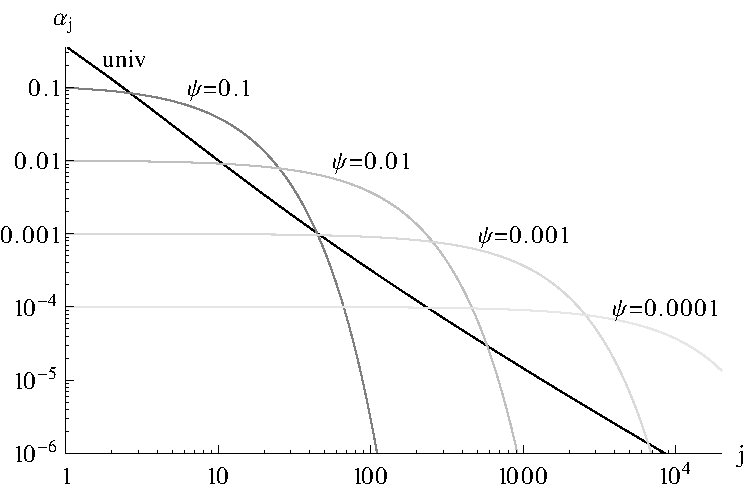
\includegraphics[width=3.5in]{figures/rules} }
 \vspace{0.2in}
 \end{figure}


%--------------------------------------------------------------------------
\section{ Risk Analysis}
%--------------------------------------------------------------------------


 Before turning to sequential estimators, we briefly review the quadratic risk
 of testimators.  We begin with the scalar case.  Let $Y \sim N(\mu,1)$.  The
 scalar testimator defined by the two-sided test of $H_0: \mu=0$ at level $\al$
 is
 \begin{equation}
   \hat\mu_\al(Y) = \left\{
     \begin{array}{cc}
        Y & \mbox{ if } z_\al^2 \le Y^2, \cr
        0 & \mbox{ otherwise, }
      \end{array} \right.
 \label{eq:muHat}
 \end{equation}
 where $z_\al$ denotes the two-sided critical value, $z_\al = \Phi^{-1}(1-\al/2)$. 
 The risk of $\hat\mu_\al$ is
 \begin{eqnarray}
   R(\hat\mu_\al(Y), \mu) 
     &=& \ev(\hat\mu_\al(Y) - \mu)^2  \cr
     &=& \mu^2 \pr(Y^2 \le z_\al^2) 
         + \int_{z_\al^2<y^2} (y-\mu)^2 \phi(y) dy \cr
     &=& B_\al(\mu) + V_\al(\mu)
 \label{eq:risk_mu_al}
 \end{eqnarray}
 The first summand $B_\al(\mu)$ is the squared bias that arises if the test of
 $H_0: \mu=0$ does not reject when $\mu \ne 0$; the second summand is the
 variance of the estimator.  Figure \ref{fig:risk}(a) shows a graph of the risk
 of testimators with $\al=0.05$ and $\al = 0.20$.  The maximum risk occurs
 near $z_\al$ and grows as $\al$ falls.  Figure \ref{fig:risk}(b) shows
 the decomposition of the risk of $\hat\mu_\al$ into $B_\al(\mu)$ and
 $V_\al(\mu)$ for $\al = 0.05$.  Because the variance component $V_\al(\mu)$
 increases smoothly to its maximum 1 for large $|\mu|$, it is the bias that
 produces the noticeable peak in the risk.


 \begin{figure}
 \caption{ \label{fig:risk} \sl The risk of a testimator peaks near $z_\alpha$ due to a
 large contribution from bias as the level $\alpha$ decreases. (a) Risk of testimators
 with $\al$ = 0.05, 0.20 versus $\mu$. (b) Squared bias and variance components of the
 risk of $\hat\mu_{0.05}$. }
 \vspace{0.1in}
\centerline{
 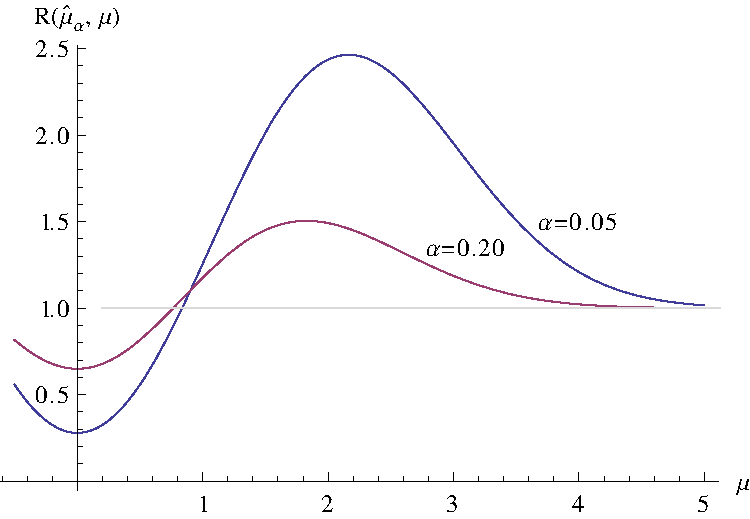
\includegraphics[width=3.0in]{figures/risk_a}
 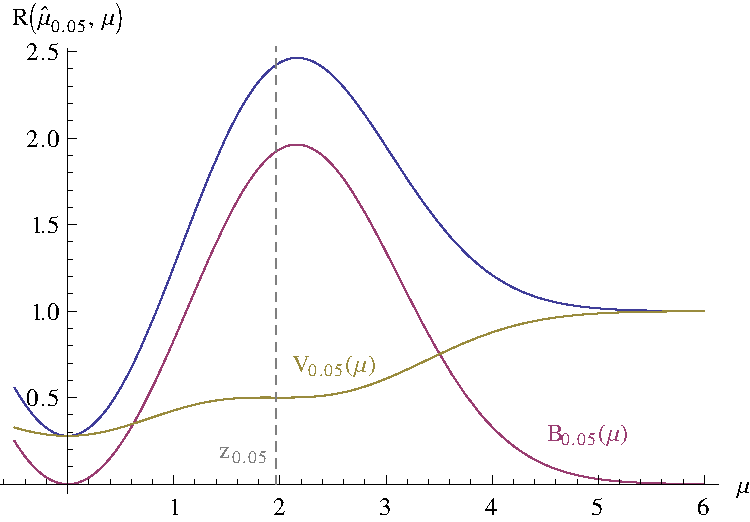
\includegraphics[width=3.0in]{figures/risk_b} }
 \vspace{0.2in}
 \end{figure}
 

 The risk of testimators is typically studied in the context of estimating a vector of $p$
 means, $\bmu \equiv \mu_{1:p} = (\mu_1, \,\ldots, \mu_p)'$.  The available data is the
 vector $\YY = (Y_1, \ldots, Y_p)'$ with distribution $\YY \sim N(\bmu,I_p)$.  In this
 context, the estimator of $\bmu$ combines testimators with a common level,
 $\hat{\bmu}_\al = (\hat\mu_\al(Y_1), \ldots, \hat\mu_\al(Y_p))'$.  The estimator
 $\hat{\bmu}_\al$ consists of zeros except for those coordinates where $z_\al^2 \le
 Y_j^2$.  The risk of $\hat{\bmu}_\al$ is the sum of the risks of the coordinate
 testimators,
 \begin{equation}
    R(\hat{\bmu}_\al, \bmu) 
      = \ev \sum_{j=1}^p \Bigl( \hat{\mu}_{\al}(Y_j) - \mu_j \Bigr)^2 \;.
 \label{eq:risk}
 \end{equation}


 Minimax bounds for the risk $R(\hat{\bmu}_\al,\bmu)$ are well-understood.  We
 review the results of \citet{fostergeorge94} who introduced the concept of the
 risk inflation of an estimator. \citet{donohojohnstone94} obtain similar results. 
 The risk inflation of $\hat{\bmu}_\al$ is the supremum of
 the ratio of the risk of $\hat{\bmu}_\al$ to that of a testimator that obtains
 the optimal level from an oracle.  Their results imply that the risk inflation
 of $\hat{\bmu}_\al$ is asymptotically about $2 \log p$,
 \begin{equation}
    2 \log p - o(\log p) 
    \le
    \sup_\mu  \frac{1 + R(\hat{\bmu}_\al,\bmu)}
                   {1 + \inf_\eta{R(\hat{\bmu}_\eta,\bmu)}}  
    \le 
    2 \log p + 1 \;.
 \label{eq:ri}
 \end{equation}
 Foster and George further show that the testimator $\hat{\bmu}_{1/p}$ --
 essentially the Bonferroni estimator -- obtains the risk inflation threshold.
  The constant 1 added to the risks in the ratio of \eqn{ri} arises in the
 context of regression models in which one always estimates the intercept.  As a
 practical device, its presence avoids dividing by zero under the complete null
 model in which $\mu_j = 0$ for all $j$.


 Though suggestive, these results do not reveal the risk of the testimator
 derived from alpha investing.  The key distinction lies in the timing of the
 information revealed in $\YY$.  The testimator $\hat{\bmu}_\al$ studied in risk
 inflation uses a fixed level $\al$ for all $p$ coordinates, and all of the
 elements of \YY are available when choosing $\al$.  In sequential testing
 controlled by alpha investing, the $Y_j$ are observed sequentially.  The
 elements of the estimator form a stochastic process, which we collect in a
 $p$-element vector as
 \begin{equation}
   \hat\mu(\al(\cdot),W_0,\omega) = (\hat\mu_{\al(W_0)}, \hat\mu_{\al(W_1)}, \ldots, 
                       \hat\mu_{\al(W_{p-1})})',
 \label{eq:muHatAlphaInv}
 \end{equation}
 where $\al(\cdot)$ denotes the defining investing rule, $W_0$ is the initial
 alpha wealth, and $\omega$ is the payout earned when rejecting a hypothesis.
  We omit $W_0$ and $\omega$ from this notation when unambiguous.
 

 The most convenient expression for the risk of \test\ relies on a recurrence.
 Let
 \begin{displaymath}
   r_\mu(\al) = \Phi(\mu-z_\al)+\Phi(-\mu-z_\al)   
 \end{displaymath}
 denote the probability of rejecting $H_0: \mu=0$ using a two-sided $z$-test at
 level $\al$ (the power of the test).  The risk of the testimator given by alpha
 investing can then be decomposed as
 \begin{eqnarray}
   R(\hat\mu(\al(\cdot),W_0,\omega),\mu_{1:p}) 
    &=& R(\hat\mu_{\al(W_0)},\mu_1)
        + \ev \sum_{j=2}^p R\Bigl(\hat\mu_{\al(W_{j-1})},\mu_j\Bigr)  \cr
    &=& R(\hat\mu_{\al_1},\mu_1)
        + r_{\mu_1}(\al_1)\; 
          R\Bigl(\hat\mu(\al(\cdot),W_0-\al_1+\omega,\omega),\mu_{2:p}\Bigr)\cr
    & & \qquad + (1-r_{\mu_1}(\al_1))\; 
          R\Bigl(\hat\mu(\al(\cdot),W_0-\al_1,\omega),\mu_{2:p}\Bigr) \;,
 \label{eq:RMuHat}
 \end{eqnarray}
 where $\al_1 = \al(W_0)$ and we have suppressed the dependence of the estimator
 on \YY.  The second expression for the risk emphasizes its recursive nature and
 motivates our method of computation.  The total risk of the estimator is the
 risk produced by the testimator for $H_1$ plus the cumulative risk of testing
 $H_2, \ldots, H_p$.  If the test of $H_1$ rejects, which happens with
 probability $r_{\mu_1}(\al_1)$, then testing the remaining hypotheses begins
 with alpha wealth $W_1 = W_0 - \alpha_1 + \omega$.  Otherwise, with probability
 $1- r_{\mu_1}(\al_1)$, testing begins with wealth $w_1 - \al_1$.


 The calculation of the maximum risk of \test\ is similarly recursive,
 and we compute the sum by backward induction.  Because the performance of
 subsequent tests depends on the outcome of the first, the choice of $\mu_1$ is
 not so simple as setting $\mu_1 = \arg \max R(\hat\mu_{0.05}, \mu)$.  Doing so
 ignores the payoff $\omega$ obtained if $H_1$ is rejected.  By rejecting the
 first test, alpha investing adds
 $\omega$ to its alpha wealth, allowing it to increase the level -- and so
 potentially reduce its risk -- in subsequent tests.  To find the maximum risk, one 
 must choose at the first test the mean
 \begin{eqnarray*}
    \mu_1 = \arg \max_{m} & \Bigl\{ & R(\hat\mu_{\al_1},m) \Bigr. 
        + r_{m}(\al_1) \; \max_{\mu_{2:p}} 
              R(\hat\mu(\al,W_0-\al_1+\omega,\omega),\mu_{2:p})\cr
    & & + \Bigl. (1-r_{m}(\al_1)) \max_{\mu_{2:p}} \; 
              R(\hat\mu(\al,W_0-\al_1,\omega),\mu_{2:p}) \Bigr\} \;.
 \end{eqnarray*}
 Notice that the sequence of means $\mu_1,\, \mu_2,\ldots, \mu_p$ that maximizes the risk is
 not deterministic because of the stochastic outcome of the tests.  As a result,
 our calculations identify a stochastic process of means that obtains, on
 average, the maximum risk.


%--------------------------------------------------------------------------
\section{ Feasible Risk Set }
%--------------------------------------------------------------------------


 Our interest is not simply in the risk of a testimator, however, but in its
 risk when compared to an alternative.  We want to see how various sequential
 testimators perform when estimating the same collection of means.  In the style
 of risk inflation \eqn{ri}, we want to contrast the risk of \test\ to that
 of another realizable testimator or to a testimator that benefits from an
 oracle that reveals $\bmu$.  The oracle-based, risk-inflation testimator
 $\tilde{\bmu}$ has elements
 \begin{equation}
   \tilde\mu_j(Y_j) = \left\{ \begin{array}{cc} 
                       0    & \mbox{ if } \mu_j^2 \le 1,        \cr
                       Y_j  & \mbox{ otherwise. }
                \end{array} \right.
 \label{eq:muTilde}
 \end{equation}
 so that its risk is 
 \begin{equation}
    R(\tilde{\bmu},\bmu) = \sum_j \min(\mu_j^2,1) \;.   
 \label{eq:riskMuTilde}
 \end{equation}
 We summarize such comparisons of risks by finding the collection of all
 possible risks that are obtainable under any mean process.  We call this
 collection the feasible risk set.  Let $\hat{\bmu}_1$ and $\hat{\bmu}_2$ denote
 two sequential estimators of $\mu_{1:p}$.  The feasible risk set for these two
 is defined as
 \begin{equation}
     {\cal R}_p(\hat{\bmu}_1,\hat{\bmu}_2) = 
      \{(r_1,r_2):  \exists \bmu \mbox{  s.t.  }
          r_1 = \evsub{\bmu} R(\hat{\bmu}_1,\bmu),\;
          r_2 = \evsub{\bmu} R(\hat{\bmu}_2,\bmu)  \} \;.           
 \label{eq:feasibleSet}
 \end{equation}
 In words, the point $(r_1,\,r_2)$ lies in the feasible set ${\cal R}_p$ if
 there exists a stochastic process of means $\bmu$ of length $p$ for which the
 risk of $\hat{\bmu}_1$ is $r_1$ and the risk of $\hat{\bmu}_2$ is $r_2$.  A
 randomization argument proves that the feasible risk set is convex.  If $x$ and
 $y$ are two points within ${\cal R}_p$, then there exist stochastic processes
 $\bmu_x$ and $\bmu_y$, say, that produce these risks.  The risk produced by the
 randomized process that picks $\bmu_x$ with probability $0 \le a \le 1$ and
 picks $\bmu_y$ with probability $1-a$ is then $a\,x+(1-a)\,y$.


 Figure \ref{fig:riFeasibleSet} shows two views of the feasible set that
 compares the risk-inflation testimator $\tilde{\bmu}$ ($x$-axis) to the universal
 testimator \uTest\ ($y$-axis).  For this figure, $p$=1,000 tests and the
 initial wealth and payout $W_0 = \omega = 0.5$.  The feasible risk set is the
 shaded region in each frame.  The feasible risk set lies above the diagonal in
 this comparison; by construction, no realizable testimator can have smaller
 risk than $\tilde{\bmu}$.  The frame on the left of Figure
 \ref{fig:riFeasibleSet} shows the feasible set on the scale of risks; the frame
 on the right shows ${\cal R}_p$ on log scales.  (${\cal R}_p$ is not
 convex on a log scale but the approximation is quite close in practice.)  We
 add 1 to the risks of both estimators, in the fashion of risk inflation, in
 order to be able to show the feasible risk set near 0 on a log-log scale.
  Points in the plot along the boundary of the feasible set identify locations
 at which we computed the exact risks using the method described in the
 following section.  Consequently, because the shaded region in the graph is
 obtained by joining these points with lines, this region is a convex subset
 within the interior of ${\cal R}_p$.  The actual risk set is slightly larger.


 \begin{figure}
 \caption{ \label{fig:riFeasibleSet} {\sl The shaded feasible set identifies the possible
 risks of the oracle estimator $\tilde{\bmu}$ and universal testimator \uTest with
 $W_0=\omega=0.5$, $p$=1,000.} The left frame emphasizes models with substantial signal;
 the right frame (log scale) highlights nearly black models. Curves within the feasible
 set show the risks as the amount of signal varies in the model \eqn{muj}. Boundary points
 show calculation locations described in Section 5; the line parallel to the diagonal in
 the right frame is the risk-inflation boundary discussed in the text.}

 \vspace{0.1in}
\centerline{
 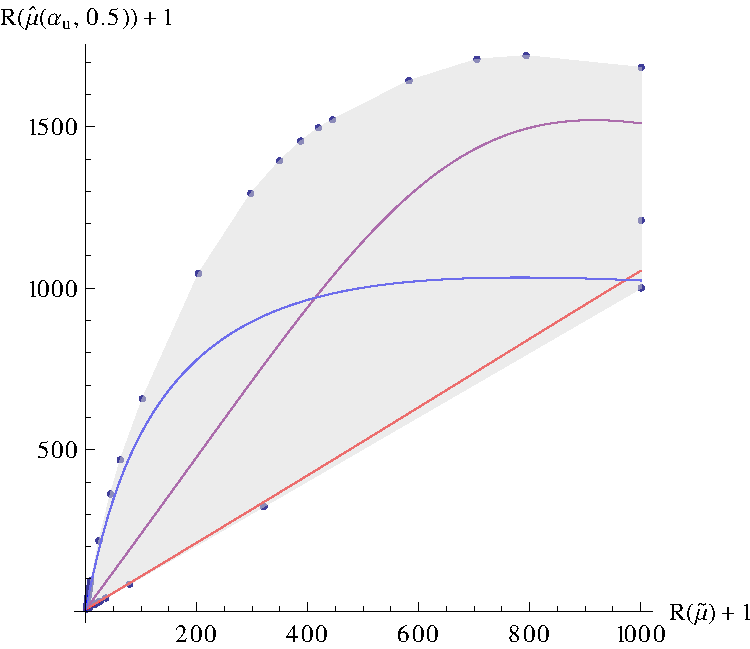
\includegraphics[width=3.0in]{figures/riFeasSet}
 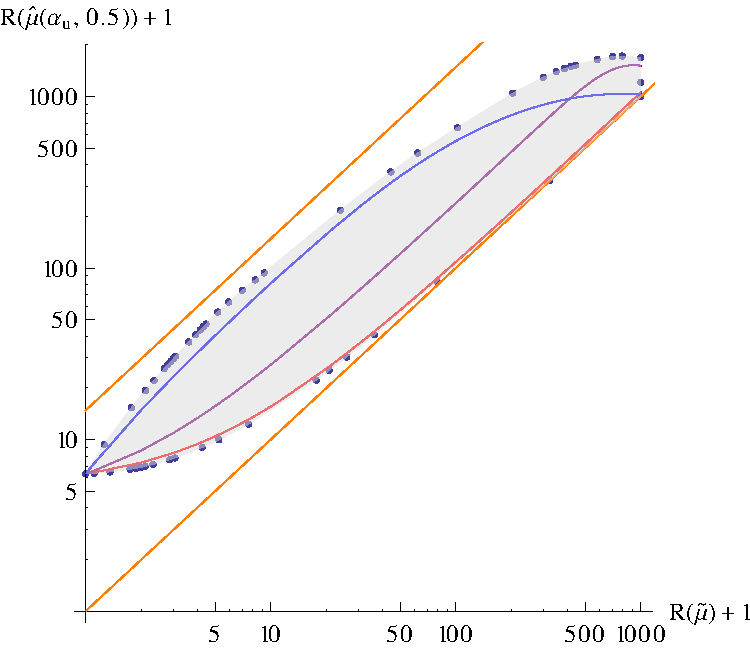
\includegraphics[width=3.0in]{figures/riFeasSetLog} }
 \vspace{0.2in}
 \end{figure}


 The two plots in Figure \ref{fig:riFeasibleSet} contrast models with substantial signal
 (non-zero means) to those that are sparse or nearly black (most $\mu_j=0$).  The frame
 scaled by the risk itself emphasizes the performance in models with substantial signal.
  The vertical right edge of the feasible set shows the risk for saturated models in which
 $|\mu_j| \ge 1$; for these models, $R(\tilde{\bmu}, \bmu) = p$.  The plot on the log
 scale emphasizes sparse models.  In this frame, the line parallel to and above the
 diagonal is the risk-inflation boundary \eqn{ri} that obtains for non-sequential
 estimators.  These bounds suggest that the worst case risk for the testimator should be
 about $2 \log p$ times the risk of the oracle.  The feasible set calculations show that
 the risk of \uTest\ does indeed fall below this boundary, but that is not true of all
 estimators.


 Curves within the feasible set shown in Figure \ref{fig:riFeasibleSet} identify the risks
 that result if $\bmu$ is determined by a two-point model.  Suppose that the stochastic
 process that determines $\bmu$ sets $\mu_j$ independently to some $\mu^{*} \ne 0$ with
 probability $\pi$ and sets $\mu_j=0$ otherwise:
 \begin{equation}
    \mu_j = B_j \; \mu^{*}, \quad B_j  \iid \mbox{ Bernoulli}(\pi)  \;.
 \label{eq:muj}
 \end{equation}
 The smooth curves within the feasible set show the risks under this model, with $\mu^{*}$
 = 1.0 (red), 1.5 (magenta), or 3 (blue), and the probability of a non-zero mean varying
 over the range $10^{-6} \le \pi \le 1-10^{-6}$.  With $\mu^{*} = 1.0$, the risks nearly
 trace out the lower boundary of the feasible set.  The crossing of the paths for
 $\mu^{*}=1.5$ and $\mu^{*}=3$ shows, however, that no one value for $\mu^{*}$ can
 reproduce the upper boundary of ${\cal R}_p$.


 Although the simple, two-point model \eqn{muj} cannot fully characterize the feasible
 set, the processes that define the boundary resemble its structure.  Figure
 \ref{fig:simRisk} graphs a realization of the stochastic process that generates the risks
 on the boundary of the feasible risk set.  For this figure, we chose the process thatcher
 produces the point with expected risks $(101, 657)$ which can be found along the left
 side of the feasible set in Figure \ref{fig:riFeasibleSet}.  The dots in Figure
 \ref{fig:simRisk} graph the elements $\mu_j$ versus the test index $j$ for $j = 1,\,2,
 \ldots, p=1,000$.  As in the two-point model, the means jump between 0 and a value that
 fluctuates around 2.63.  The increasing trend in the figure shows the cumulative risk
 obtained by the universal testimator for this realization.  Its risk in this instance
 reaches 688, whereas the cumulative risk of the oracle is 123.


\begin{figure}
 \caption{ \label{fig:simRisk} {\sl The mean process associated with a boundary point of 
 the feasible set produces realizations that resemble those of the two-point model 
 \eqn{muj}.} The increasing trend shows the accumulating risk of the testimator 
 which reaches 688 in this example.  }

 \vspace{0.1in}
 \centerline{
 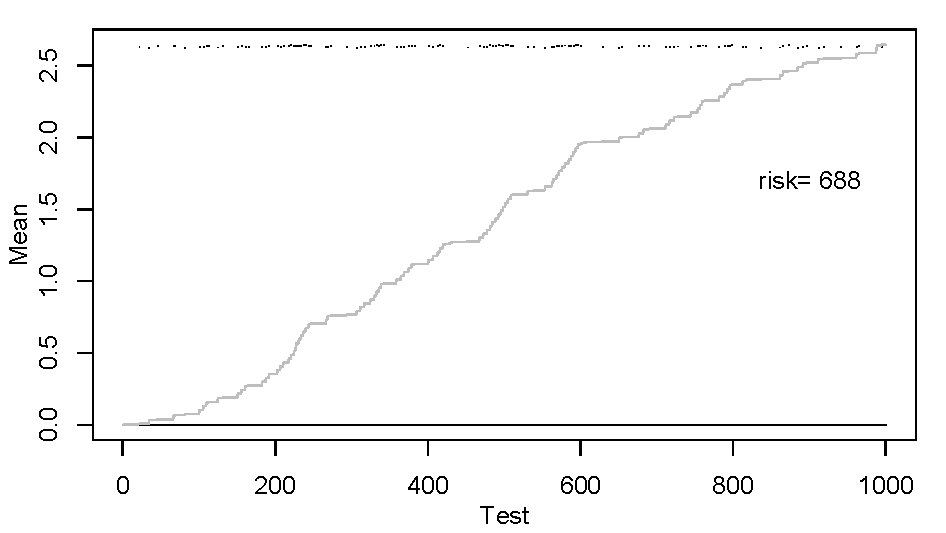
\includegraphics[width=3.5in]{figures/simRisk}    }
 \vspace{0.2in}
\end{figure}


 Displays that combine several feasible sets allow one to compare the effects of various
 choices for $W_0$ and $\omega$.  As an example, Figure \ref{fig:univRI} considers the
 effect of reducing the initial wealth $W_0$ and payoff $\omega$ from 0.50 down to 0.25
 and 0.05.  As before, the left frame emphasizes estimation with greater levels of signal;
 the right frame on the log scale emphasizes sparse models.  Within the context of
 hypothesis testing, $\al=0.05$ is a virtual default and one may be similarly tempted to
 control mFDR at 0.05.  Unless one believes that nature will play a nearly black strategy,
 however, setting $W_0 = \omega = 0.05$ generates greater risk than $W_0=0.25$ or 0.50.
  With $W_0=0.05$, the risks even escape the bounds suggested by risk inflation in the
 non-sequential setting, shown here by a portion of the feasible set above the bound
 provided in \eqn{ri}.
 
 \remark{ Because the plots in Figure
 \ref{fig:univRI} show several feasible sets together, one can no longer
 associate a point in the graph with a single mean process $\bmu$.
  Points within each feasible set indicate that
 there exists a mean process that generates the shown risks, but at a given
 $(x,y)$ location, the mean processes that produce the risks for the feasible sets
 may differ.}


\begin{figure}
 \caption{ \label{fig:univRI} {\sl The initial wealth and payout influence the 
  feasible set of risks that contrast the risk-inflation testimator $\tilde\bmu$  to the universal estimator
 \uTest.} The initial wealth varies over $W_0=0.05$,
 0.25, and 0.50 with $p$=1,000 tests on the scale of risks (left) or log risks
 (right).  }

 \vspace{0.1in}
 \centerline{
 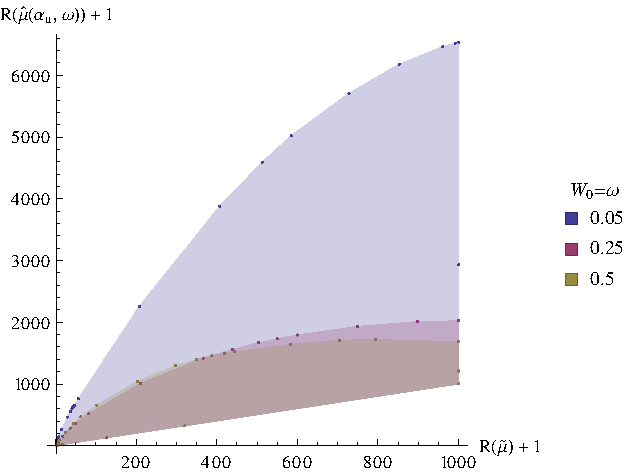
\includegraphics[width=3.5in]{figures/univVsRI}
 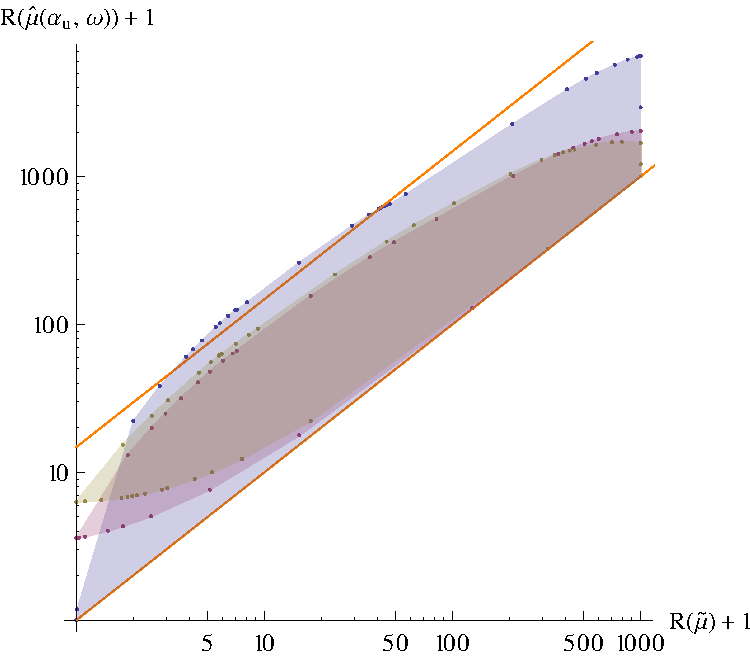
\includegraphics[width=3.0in]{figures/univVsRILog}    }
 \vspace{0.2in}
\end{figure}


 We have emphasized universal investing defined by $\al_u$, and Figure
 \ref{fig:geo} offers a partial explanation for our preference.  Figure \ref{fig:geo}
 superimposes the feasible sets obtained by geometric investing with various rates versus
 the risk-inflation testimator $\tilde\bmu$.  The results are for a sequence of $p = 500$ tests.  In
 general, increasing the spending rate $\psi$ from 0.001 up to 0.01 reduces the risk of
 the geometric testimator $\al_g(w,\psi)$. The feasible sets for $\psi=0.001$, 0.005, and
 0.01 progressively concentrate toward the diagonal, better competing with $\tilde\bmu$.  
 The move to $\psi = 0.05$, however, goes too far.  The geometric estimator
 essentially exhausts its alpha wealth before the testing is complete, and consequently
 its risk soars.  Because this geometric estimator essentially sets $\hat\mu_j \equiv 0$
 as its alpha wealth approaches 0, its risk exceeds the risk inflation boundary
 \eqn{ri}.


\begin{figure}
 \caption{ \label{fig:geo} {\sl A high spending rate $\psi$ potentially exhausts the
 wealth of a geometric testimator and produces excessive risks compared to $\tilde\bmu$.}
  These results are for $p=500$ tests and rates $\psi=$ 0.001, 0.005, 0.01, and 0.05.  }

 \vspace{0.1in}
 \centerline{
   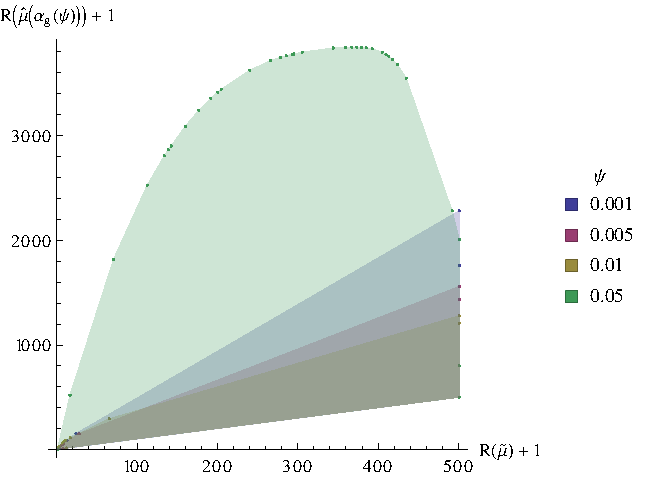
\includegraphics[width=3.5in]{figures/geom}     }
 \vspace{0.2in}
\end{figure}


 As a final example, feasible risk sets also allow us to directly compare
 realizable testimators produced by different methods of alpha investing.
  Rather than compare a realizable testimator to an oracle
 as in Figures \ref{fig:univRI} and \ref{fig:geo}, the feasible set ${\cal R}_p (\hat\mu(\al_u),
 \hat\mu(\al_g))$ shown in Figure \ref{fig:univGeo} pits these two against each
 other in a head-to-head comparison.  The initial value and payout for both are
 $W_0 = \omega = 0.25$.  The rates of the geometric strategy are set to
 $\psi=0.001$, 0.002, and 0.005.  Small rates are necessary to avoid the surge
 in risk illustrated in Figure \ref{fig:geo} when the geometric strategy runs
 out of wealth.  There are clearly mean processes for which either choice,
 universal or geometric, dominate the other.  That said, this figure clarifies
 the relative advantages of universal investing over geometric investing.  
 A higher investing rate $\psi$ for geometric investing
 reduces risk for models with more signal, but doing so necessarily leads to
 higher risks in nearly black models.  For instance, the set in Figure
 \ref{fig:univGeo} associated with $\psi = 0.005$ reduces the bulge toward higher
 risks in the left frame, but this choice is soundly dominated by slower
 spending rates in models with fewer non-zero parameters emphasized by the log scale
 in the right frame.  Universal investing removes this tuning parameter.


 \begin{figure}
 \caption{ \label{fig:univGeo} {\sl The universal alpha investing testimator
 \uTest\ (y-axis) produces typically smaller risks than geometric testimators
 \gTest\ (x-axis).}  The geometric rates are $\psi = 0.001$, 0.002, and 0.005 with
 $p=$1,000.}

 \vspace{0.1in}
 \centerline{
     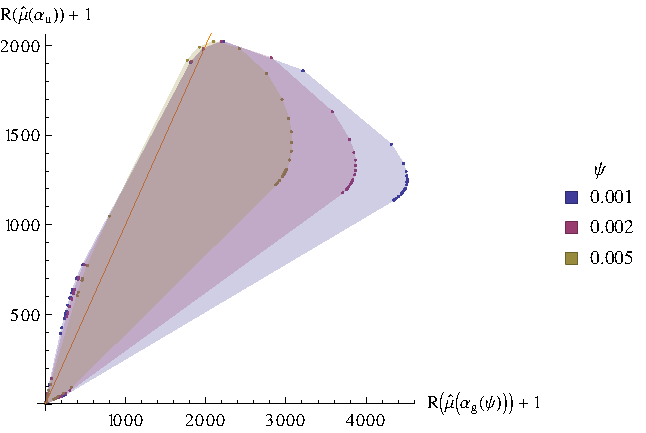
\includegraphics[width=3.5in]{figures/univGeo}
     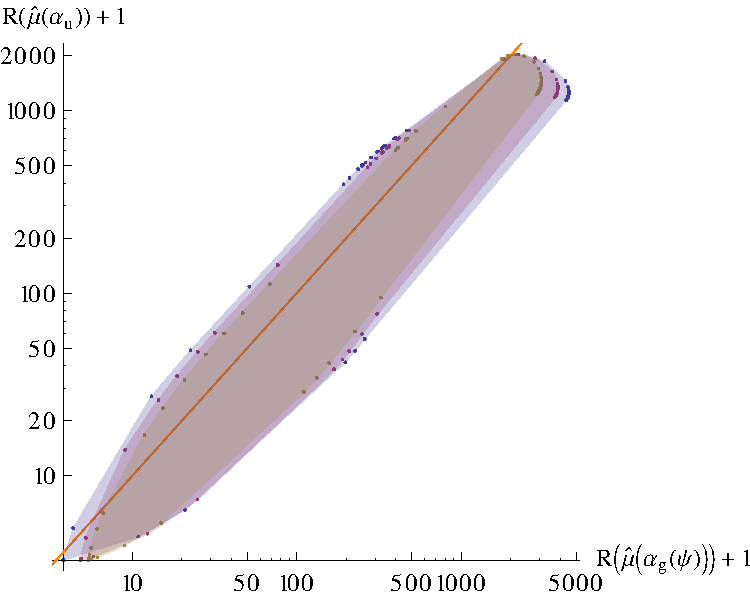
\includegraphics[width=2.9in]{figures/univGeoLog} }
 \vspace{0.2in}
 \end{figure}



%--------------------------------------------------------------------------
\section{ Computation }
%--------------------------------------------------------------------------

 We describe first the calculation of the feasible set ${\cal R}_p(\hat\mu(
 \al(\cdot), W_0, \omega), \tilde{\bmu})$ that contrasts an alpha investing
 testimator with the risk-inflation testimator $\tilde\bmu$.  Because $\tilde\bmu$
 has no wealth constraint, calculations need only track
 the wealth of the alpha investing estimator, which we abbreviate as
 $\hat{\bmu}$ with the understanding that it depends on the choice of the
 investing function $\al(\cdot)$, $W_0$, and $\omega$ throughout this section.
  Let
 \begin{equation}
   {\cal U}^\theta(\hat{\bmu},\tilde{\bmu}) = 
       \max \evsub{\bmu} \Bigl(
       \cos(\theta) R(\hat{\bmu}, \bmu) + \sin(\theta) R(\tilde{\bmu},\bmu) 
       \Bigr)
 \label{eq:U}
 \end{equation}
 denote the maximum expected value with respect to a stochastic process $\bmu$
 of the weighted sum of risks defined by the angle $ 0 \le \theta \le 2 \pi$.
  Let $\bmu^\theta$ denote the mean process that maximizes ${\cal U}^\theta$.  The
 point $\evsub{\bmu^\theta}(R(\hat{\bmu}, \bmu), R(\tilde{\bmu}, \bmu))$ lies on
 the boundary of ${\cal R}_p(\hat{\bmu},\tilde{\bmu})$ where the feasible risk
 set is tangent to the line defined by the mixture weights in \eqn{U}.  Plots
 that show the feasible risk set, such as Figure \ref{fig:riFeasibleSet},
 highlight the boundary points that are explicitly computed.  By varying
 $\theta$ over the circle, we approximate the feasible risk set as the
 intersection of the resulting half-planes.

 
 We compute ${\cal U}^\theta$ via numerical backward induction.  This induction
 approximates the wealth of the alpha investing testimator on a grid.  The
 wealth grid $G$ reaches from the minimal attainable wealth ($W_0 - \sum_{j=1}^p
 \al_j$) to a maximum allowed wealth, which we set to $W_{\max} = 5$.  (Our
 results have not been sensitive to the choice of $W_{\max}$ so long as it is
 substantially larger than $W_0 + \omega$.)  The wealth grid is
 `logarithmically' spaced at $N$ points, with a finer spacing 0.0001 for small
 wealths below 0.001 and gradually larger spacing as the wealth increases.  We
 insure that the grid includes an element $G_{k_0} = W_0$.


 The $p \times N$ matrix $U^{\theta}$ holds intermediate calculations of the
 expected value ${\cal U}^{\theta}$.  The rows in this matrix identify the hypothesis $H_j$
 and the columns index the position in the wealth grid $G$.  We fill $U^\theta$
 from the `bottom up' in a tail recursion.  At the completion of the
 calculations,
 \begin{eqnarray}
   U^\theta_{jk} &=&  \max_\mu \;\Bigl\{
     \cos(\theta) R(\hat\mu_{\al(G_k)}, \mu) + \sin(\theta) R(\tilde{\mu},\mu) \cr
     & &+ r_\mu\left(\al(G_k)\right) \;
          \left(c \,U^{\theta}_{j+1,k_c+1} + (1-c) U^{\theta}_{j+1,k_c}\right) \cr
     & & + \left(1- r_\mu(\al(G_k))\right) \; 
          \left(d \,U^{\theta}_{j+1,k_d+1} + (1-d) U^{\theta}_{j+1,k_d}\right)   
     \Bigr\}
 \label{eq:Ujk}
 \end{eqnarray}
 for $j=p, p-1,\ldots,1$ and $k = 1,\ldots,N$ and the boundary condition
 $U^\theta_{p+1,k} = 0$.  Note the similarity to expression \eqn{RMuHat}.  At
 the completion of the computation, ${\cal U}^\theta = U^{\theta}_{1,k_0}$.  The
 first line of \eqn{Ujk} adds the contribution to the weighted risk from
 testing $H_j$ at the alpha level $\al(G_k)$.  The second line adds the expected
 subsequent risk if the test rejects $H_j$, which occurs with probability
 $r_\mu(\al(G_k))$.  If the test rejects, the alpha wealth increases to $G_k -
 \al(G_k) + \omega$.  This wealth is unlikely to match that at any grid
 position, so we linearly interpolate between positions $k_c$ and $k_c+1$ so
 that $G_{k_c} \le G_k - \al(G_k) + \omega \le G_{k_c+1}$ and set the weight $c$
 in \eqn{Ujk} to $c = (G_k - \al(G_k) + \omega)/(G_{k_c+1}-G_{k_c})$.
  Similarly, the third line of \eqn{Ujk} adds the expected contribution if
 the testimator does not reject $H_j$ and its wealth falls to $G_k - \al(G_k)$.

 \remark{ One need not store the full matrix $U^\theta$, but its use simplifies
 the description of the algorithm.  One only needs the next row $U^\theta_{j+1,
 \cdot}$ to compute $U_{j,\cdot}$.  Such space saving -- using just two rows
 rather than the full matrix -- becomes essential in problems that track a
 larger state space.  Note also that one can cache the indices and weights
 ($k_c, c$ and $k_d, d$) prior to the recursion because these can be determined
 from the grid positions and $\omega$ and remain fixed throughout the backward
 recursion.}


 The feasible set that compares the testimators defined by two alpha investing
 rules $\al(\cdot)$ and $\beta(\cdot)$ requires a more complex recursion that
 must track the wealths of both.  The linear grid $G$ remains, but the matrix
 $U^\theta$ defined in \eqn{Ujk} becomes a three dimensional tensor of size
 $p \times N \times N$.  The calculation is essentially a more messy version of
 \eqn{Ujk} but for one nuance that we want to emphasize.  To simplify the
 presentation, we suppress the linear interpolation and pretend that all of the
 concerned wealths are represented in the wealth grid.  If the alpha investing
 rule $\al(\cdot)$ with wealth $G_k$ rejects $H_j$, its wealth goes from $G_k$
 to $G_{k+}$; if it fails to reject, its wealth falls to $G_{k-}$.  Similarly,
 we use $\ell+$ and $\ell-$ for the positions for the rule defined by
 $\beta(\cdot)$.  If we assume $\al(G_k) < \beta(G_\ell)$, then the recursion
 can be written as
 \begin{eqnarray}
   U^\theta_{jk\ell} &=&  \max_\mu \;\Bigl\{
     \cos(\theta) R(\hat\mu_{\al(G_k)}, \mu) 
       + \sin(\theta) R(\hat\mu_{\beta(G_\ell)},\mu) \cr
     & & + r_\mu\left(\al(G_k)\right) \; U_{j+1,k+,\ell+} 
         + \left[ r_\mu(\beta(G_\ell)) - r_\mu(\al(G_k)) \right] \, U_{j+1,k-,\ell+} \cr
     & & + \left[1-r_\mu(\beta(G_\ell))\right] \, U_{j+1,k-,\ell-} \, \Bigr\}\;,
 \label{eq:Ujkl}
 \end{eqnarray}
 where the boundary condition is $U_{p+1,\cdot,\cdot}^\theta= 0$.  The first
 line in \eqn{Ujkl} is the expected risk produced by the test of $H_j$, and
 following summands denote the expected contributions to the risk if both
 reject, if only the rule with the larger alpha level rejects, and if neither
 rejects.  The point of writing this out is to emphasize these testimators see
 the same data, not independent samples.  Hence, $\al(G_k) < \beta(G_\ell)$
 implies that if the first rule $\al(\cdot)$ rejects $H_j$, then the second rule
 must also reject $H_j$ because it tests the same hypothesis using the same
 data, but with a larger alpha level.


%--------------------------------------------------------------------------
\section{ Discussion }
%--------------------------------------------------------------------------

 Feasible risk sets allow us to study the risks of testimators in sequential problems.
  The comparisons shown here suggest that universal alpha investing does well and can
 compete with the risks attained by any geometric procedure.  It is also of interest to
 point out that a large initial alpha wealth and payout $W_0 = \omega = 0.25$ produce a
 noticeable reduction in the risk (Figure \ref{fig:univRI}).  This choice for $\omega$
 implies that controlling the expected false discovery rate at 25\%, quite a bit larger
 than would usually be chosen, produces lower risk unless the mean process is quite
 sparse.  For example, the comparisons of streaming estimators in \citet{wu13} set $W_0$
 and $\omega = 0.01, 0.05$.  It would be useful to investigate whether larger choices
 improve the performance of these estimates in their models (which are more complex than
 the idealized testing of independent means shown here).


 A particular benefit of these computations is that they suggest conjectures
 about asymptotic properties of these estimators.  For example, it appears that
 we can approximate the boundary of the feasible risk set using two-point models
 defined in \eqn{muj}.  Figure \ref{fig:riFeasibleSet} shows that by varying
 the signal probability $\pi$ such a model can be found that approaches the
 boundary of the feasible risk set.  Further, the simulation shown in Figure
 \ref{fig:simRisk} shows that (at least for this location) the boundary mean
 process generates either zero or approximately a single, non-zero value.
  Hence, it would appear that, asymptotically in $p$, there exists a two-point
 model $(\pi,\,\mu^{*})$ for which the risks lie within some epsilon ball of the
 boundary of the feasible risk set.


 The shapes of the various feasible sets are also intriguing.  For instance in
 Figure \ref{fig:riFeasibleSet}, the set has a vertical segment where the risk
 of the oracle attains its maximum at $p$.  These risks occur when the mean
 process is saturated in the sense that every $\mu_j^2 \ge 1$ so that the
 risk-inflation oracle ``fits everything.''  Although the oracle then has fixed
 risk $p$, the risk of the testimator varies with the size of $\mu_j$.  This
 property of the feasible risk set for saturated mean processes is rather
 different from the behavior for sparse processes.  As the risk of the oracle
 estimator approaches its minimum, the feasible risk set approaches a single
 point.  That the set comes to a point is not surprising.  Unlike the saturated
 case, a unique process produces the minimum risk, namely the process for which
 every $\mu_j = 0$.  What is surprising is the lack of evident curvature.  Does
 the feasible set come to a point or instead form a very tight curve?
 

 As a final conjecture, the performance of testimators derived from the
 universal rule $\al_u(\cdot)$ suggests that this investing rule can simplify
 the choice of an alpha investing method.  Figure \ref{fig:univGeo} shows its
 ability to match the risks obtained by various geometric testimators.  Ideally,
 we would like to obtain results that show that universal alpha investing is about
 as good as one can do, analogous to those in \citet{rissanen83}.  Such a proof would
 then simplify the use of alpha investing in practice as one would not need to
 struggle with the choice of an investing rule but instead could focus on
 generating a better stream of features.


%--------------------------------------------------------------------------
\section*{Appendix}
%--------------------------------------------------------------------------

 We obtained the universal rule $\al_u$ defined in \eqn{Auniv} by
 the following construction.  The idea is to define a spending rule by a
 probability distribution that allocates wealth over subsequent tests and then
 shift from discrete to continuous distributions.  We illustrate the
 construction for the geometric rule.  If the initial wealth is $W_0$, then the
 alpha wealth invested in the $j$th test (assuming no intervening test rejects)
 is
 \begin{equation}
    \al_j = W_0\; \psi \; (1-\psi)^{j-1} \;, \quad j = 1, 2, \ldots\;.   
 \label{eq:alj1}
 \end{equation}
  Rather than define the investing rule using a discrete distribution on
 $j=1,\,2,\ldots$ as in \eqn{alj1}, consider the continuous density
 \begin{equation}
   A_g(x) = c_g \; \psi\,(1-\psi)^{x-1}, \quad 1 \le x\;,
 \label{eq:alg}
 \end{equation}
 where the normalizing constant $c_g = -\log (1-\psi)/\psi$ implies
 $\int_1^{\infty} A_g(x) dx = 1$.  Notice that the wealth invested in the $j$th
 test \eqn{alj1} matches $W_0$ times the integral of $A_g(x)$ from $x=j$ to
 $j+1$,
 \begin{equation}
    \al_j = W_0 \int_j^{j+1} A_g(x) dx = W_0 \, \psi\; (1-\psi)^{j-1} \;.
 \label{eq:alj2}
 \end{equation}
 To move away from discrete indexing, we use the following tail integral,
 \begin{equation}
    W_g(x) = W_0 \int_x^\infty A_g(t,\psi) dt = W_0 (1-\psi)^{x-1}\;.
 \label{eq:Wg}
 \end{equation}
 For integers $j$, $W_g(j)$ is the wealth available to test $H_j$ if none of
 $H_1$, $H_2, \ldots,\, H_{j-1}$ are rejected.  By inverting this tail integral,
 we can write the investing rule as a function of just the available wealth,
 \begin{equation}
   \al_g(w,\psi) = A_g(W_g^{-1}(w)) = \psi\,w \;,
 \label{eq:Ag}
 \end{equation}
 as in \eqn{Ageo}.  This construction uses the inverse of the tail wealth to
 determine a `hypothesis index' $W_g^{-1}(w)$ that corresponds to wealth $w$.
  The universal rule $\al_u(w)$ follows from the same construction, but starts
 with the density $A_u$ defined in equation \eqn{Au}.
 

%--------------------------------------------------------------------------
\section*{Acknowledgement}
%--------------------------------------------------------------------------

 The authors gratefully acknowledge support from NSF (award \#1106743) and the helpful
 suggestions from an anonymous referee.


%--------------------------------------------------------------------------
% References
%--------------------------------------------------------------------------

\bibliography{../../../../references/stat}
\bibliographystyle{../../bst/asr}

\end{document} %==========================================================

% LocalWords:  jk
